%%%%%%%%%%%%%%%%%%%%%%%%%%%%%%%%%%%%%%%%%%%%%%%%%%%%%%%%%%%%%%%%%%%
%                                                                 %
%                            CHAPTER ONE                          %
%                                                                 %
%%%%%%%%%%%%%%%%%%%%%%%%%%%%%%%%%%%%%%%%%%%%%%%%%%%%%%%%%%%%%%%%%%%

\chapter{INTRODUCTION}

\section{Introduction}
Anyone who has used an iPhone or owned a video game console understands the basics of versioning.
Companies brand sequential devices to indicate improvements in performance or capabilities.
This basic identification method has given rise to a plethora of versioning systems used widely across a landscape of software and data.
They help scientific workflows avoid losing work by managing transitions and changes while in operation \cite{Casati1996}.
They provide necessary documentation which informs the transition to new methods and procedures \cite{Wiil:2000:RDH:338407.338517}.
They provide accountability for the value of a project's data set when considering an agency's continued funding \cite{Cavanaugh2002}.
As Barkstrom writes in 2003,
\begin{quotation}
	If scientific data production were easy, instruments would
	have stable calibrations and validation activities would discover no need for
	corrections that vary with time. Unfortunately, validation invariably shows that
	instrument calibrations drift and that algorithms need a better physical basis.
\end{quotation} \cite{Barkstrom2003}.
The natural evolution of these systems, however, have given rise to formal architecture operating on top of very informal concepts.
In this dissertation, we identify gaps in versioning practices which result from tradition and develop a data model to more completely capture the interactions involved in versioning.

\section{Definitions of Version}

Using versions in the vernacular has become so pervasive that few documents formally define it.
Barkstrom describes versions as \textbf{homogeneous groupings} used to control, ``production volatility induced by changes in algorithms and coefficients as result of validation and reprocessing," \cite{Barkstrom2003}.
This definition's first implication is that such \textbf{groupings} indicate an expectation that versioning requires multiple objects.
With only one object, all metadata would be homogeneous and \textbf{groupings} would become unnecessary.
Whether in the same or different groups, the relationship between entries informs the \textbf{grouping} necessary to organize the data collection.
Figure \ref{hierarchy} visually displays this concept with each file having a clearly defined \textbf{grouping} at each hierarchical level.
Another implication is that version changes can be determined by studying the difference in provenance between two objects.
Changes in algorithms and coefficients may induce enough volatility into the data that a new \textbf{grouping} becomes necessary.
However, this relies heavily on knowing which provenance changes correspond with resulting volatility.
A new version of a data set can result from modifications to data downstream propagated through a workflow without significant changes to the immediate algorithm or coefficients.
In addition, a deeper investigation would become necessary to quantify the amount of volatility introduced by these changes, and how much is necessary to induce a change at each level of the hierarchy.
Therefore, a version definition cannot rely on provenance alone.

Another definition comes from Tagger in which versions are a, ``semantically meaningful snapshot of a design object," \cite{Tagger2005}.
Unfortunately, he does not further clarify what he means by semantically meaningful.
It is, however, important to note that these snapshots are not of any design object, but the same one.
A similar context connects each snapshot, meaning that they are versions as a result of sharing the same subject and setting.
More specifically, these designs perform the same function in their application.

Combining these conclusions together, a clearer image emerges.
A \textbf{version} is, at its core, a work, but it is not a singular work.
\textbf{Versions} are members of a group which have common, but varying provenance.
However, these members must also perform the same function as others in their group.
This creates specific requirements as to when two objects can be considered \textbf{versions} of each other.

Notice that neither definition includes how to generate versions.
The derivation, PROV Ontology's analog for a version, is defined as, ``a transformation of an entity into another, an update of an entity resulting in a new one, or the construction of a new entity based on a pre-existing entity," \cite{Lebo2013}.
In this view, a \textbf{version} exists because an activity generated it.
However, looking more closely at the forces acting upon the \textbf{version}, they generate an object which becomes a derivation of another as a result of sharing the properties previously mentioned.
The version identifier becomes applied using prior knowledge, not as a result of generation activities.
That is, an activity determines whether an object is a version of another based on the state of that object.
Therefore, \textbf{versioning} is the activity of identifying two objects connected by provenance and exposing the changes relating them, not of generating versions.

\section{Version Systems}

Many text-based data sets rely on well-established algorithms to perform this alignment  \cite{Chien:2000:VMX:646544.696357}.

Clotho, a versioning application managing versions at the block level, coordinates constrained spaces using intermittent compact and un-compact methods when retrieving or storing old objects \cite{Flouris04clotho:transparent}.

Collection into larger unified repositories will likely require a multi-tiered approach to synchronize the varied practices  \cite{Baker2009}.
Baker notes that differences depend on the sociotechnical distance of a repository from the data's origin \cite{Baker2009}.
Local stores closer to the collection site better understand data capture conditions, but must also adapt to changing environments.

Likewise, many version control tools include functions to display the versioning tree, but this is also an ease-of-use function \cite{Dijkstra1994}.

\cite{Stuckenholz:2005:CEV:1039174.1039197} - Component Evolution and Versioning State of the Art
The setup proves ideal for data sets which prioritize service to their most recent versions \cite{Stuckenholz:2005:CEV:1039174.1039197}.

Some methods like the inverted file index have been developed to balance space and retrieval performance on web documents, especially since wikis and news feeds have grown in deployment \cite{Berberich:2007:TMT:1277741.1277831}.

This proves increasingly important as the ability to propagate relevant data change across autonomous systems then assures valid quality in interactions between domains \cite{Systems02champagne:data}.

\subsection{Library Sciences}

Data on a hurricane sometimes occupy only a small portion of a data set, and the files may not even be adjacent in the collection \cite{Barkstrom_digitallibrary}.

Libraries curate multiple editions of the same work, sometimes with significant revisions \cite{Wiil:2000:RDH:338407.338517}.

Data managers often impose a sequential ordering in conjunction with logical groupings to form an object's historical lineage \cite{barkstrom2014earth}.

However, for many library or catalog environments, they cannot predict the target volume a user desires and must prioritize availability \cite{Payette2002} \cite{Barkstrom_digitallibrary}.

However, different data sets may utilize each of the three core operations at different rates \cite{rohtua}.

\subsection{Software Versioning}

Software versioning tools like RCS commonly feature branching and merging functions to create a versioning line separate from the stable master branch \cite{tichy1985rcs}.

The software manager GIT employs this method and Figure \ref{GITFile} demonstrates an example storage space for multiple versions \cite{Chacon:2009:PG:1618548}.

\begin{figure}
	\centering
	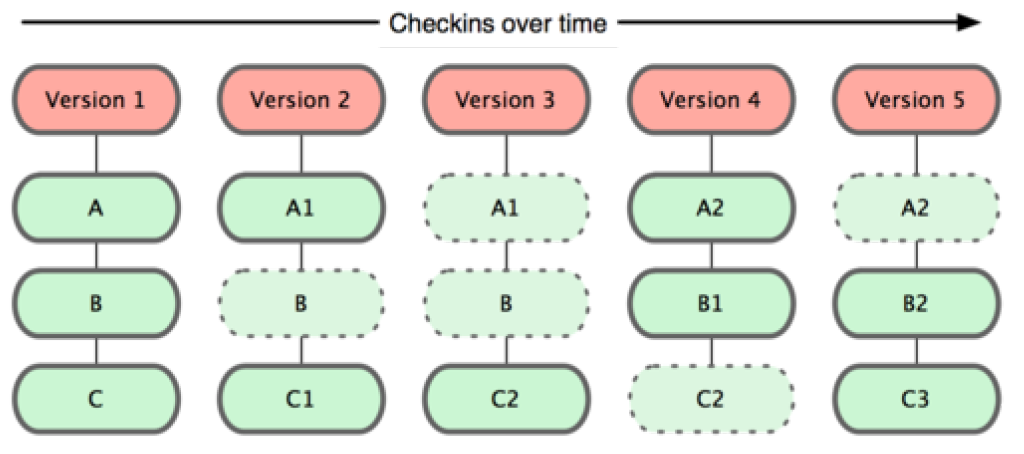
\includegraphics[scale=0.50]{figures/GITFiles.png}
	\caption[GIT stores changes in the repository as snapshots of individual files.]{GIT stores changes in the repository as snapshots of individual files. Figure 1.5 from \cite{Chacon:2009:PG:1618548}}
	\label{GITFile}
\end{figure}

Using identifiers to convey extended versioning information becomes more difficult with the adoption of distributed version managers like GIT \cite{cederqvist2002version}.

\subsection{Database Versioning}

As data sets continue to grow in size, it may become impractical to look towards data as the driving source for identifiers, as Proell and Rauber suggest that database queries may provide a more scalable means of citing data sets \cite{proellBigData}.

This gave rise to the first temporal databases where schemas included time and dated transactions modifying the schema \cite{roddick1996model}.

Fischer, et al., demonstrate the importance of having a regular standardized version identification system, as it provides a mechanism to track errors being addressed \cite{Fischer2003}.

Klahold, et al., introduced using abstract versioning environments to separate the temporal features and organize them into related groupings \cite{Klahold:1986:GMV:645913.671314}.

As publications more often include citations to data, researchers adjust to enormous modern databases with new methods changing queries rather than transforming schemas \cite{Proell2013} \cite{DBLP:conf/data/2013}.

However, massive centralized data stores have become more prevalent as data distribution methods advance  \cite{Vassiliadis1999}.

\subsection{Grid Versioning}

However, users do not have this advantage and system managers are starting to recognize the difference in versioning usage patterns between users and producers \cite{Branco2008}.

This seems to be a recurring cycle of attention with rapidly developing technologies such as the grid or parallel computing \cite{Kovse2003VGridAVS}.

The CERN grid for the Compact Muon Solenoid experiment carefully developed necessary processes which allow references by multiple users to the same file without copying that file across the grid \cite{Holtman:687353}.

This behavior becomes entirely too slow as data providers begin allowing users to dynamically generate data products from existing data according to their needs \cite{Barkstrom2003a}.

\subsection{Ontology Versioning}

\cite{HauptmannEtAl:LDQ2015} \cite{LDQ2015} - Scalable Semantic Version Control for Linked Data Management

Klein and Fensel determined versioning systems needed to capture compatibility as a major characteristic while performing a study of different ontology versioning methods \cite{Klein01ontologyversioning}.

Take, for example, some biological ontologies, which must update terms and definitions to better capture the field \cite{Ochs:2015:SVS:2826733.2826866}.

Many text-based data sets rely on well-established algorithms to perform this alignment  \cite{Hartung201315}.

\section{Version Models} \label{sec:models}

Properly detecting changes in a system's files allows file managers to correctly group them into versions as seen in research conducted by the Atmospheric Radiation Measurements (ARM) group \cite{6906868}.

Initial research in version modeling occurred with databases, studying ways to track and migrate schema changes.
Capturing periodic snapshots or copies becomes unfeasible with increasingly large centralized database systems.
This provides the database a method to transactionally rollback the environment to recreate a search.
As databases grew more complex, the intricate relationships between objects made rollbacks more difficult.
This results from the need to manage the time instances of realization, storage, and validity.
The datum becomes realized at collection, then stored upon entry into the database, and finally valid until the present or new data replaces it.
This method, however, relies on an abstract model capturing data changes to inform query modifications.

Data models allow the capture of complicated relationships between data objects within a system without needing to physically look over sizable data sets.
However, as discussed previously, versioning seeks to expose relationships between objects which may not describe how to construct either one.
The Health Care and Life Sciences (HCLS) Interest Group of the World Wide Web Consortium (W3C) recently released a model which may provide a solution when used in conjunction with other identifiers \cite{Dummontier2016}.
Their model, shown in Figure \ref{HCLSModel}, separates the concept of a data set into three groupings.
The highest level summarizes the data as an abstract work, perhaps better described as a topic or title.
This data topic can have multiple versions as it changes over time.
The version can then be instantiated into various distributions with different formats.
Compare this to the diagram in Figure \ref{hierarchy} which features more tiers.
In this case, the basis for diverging groups is changes in identifier and physical formating of that version.
This model also demonstrates how it can better communicate scientific similarity than an identifier.
The model logically links together, under a single version, representations of that data adjusting for physical perturbations.

\begin{figure}%[b]
	\centering
	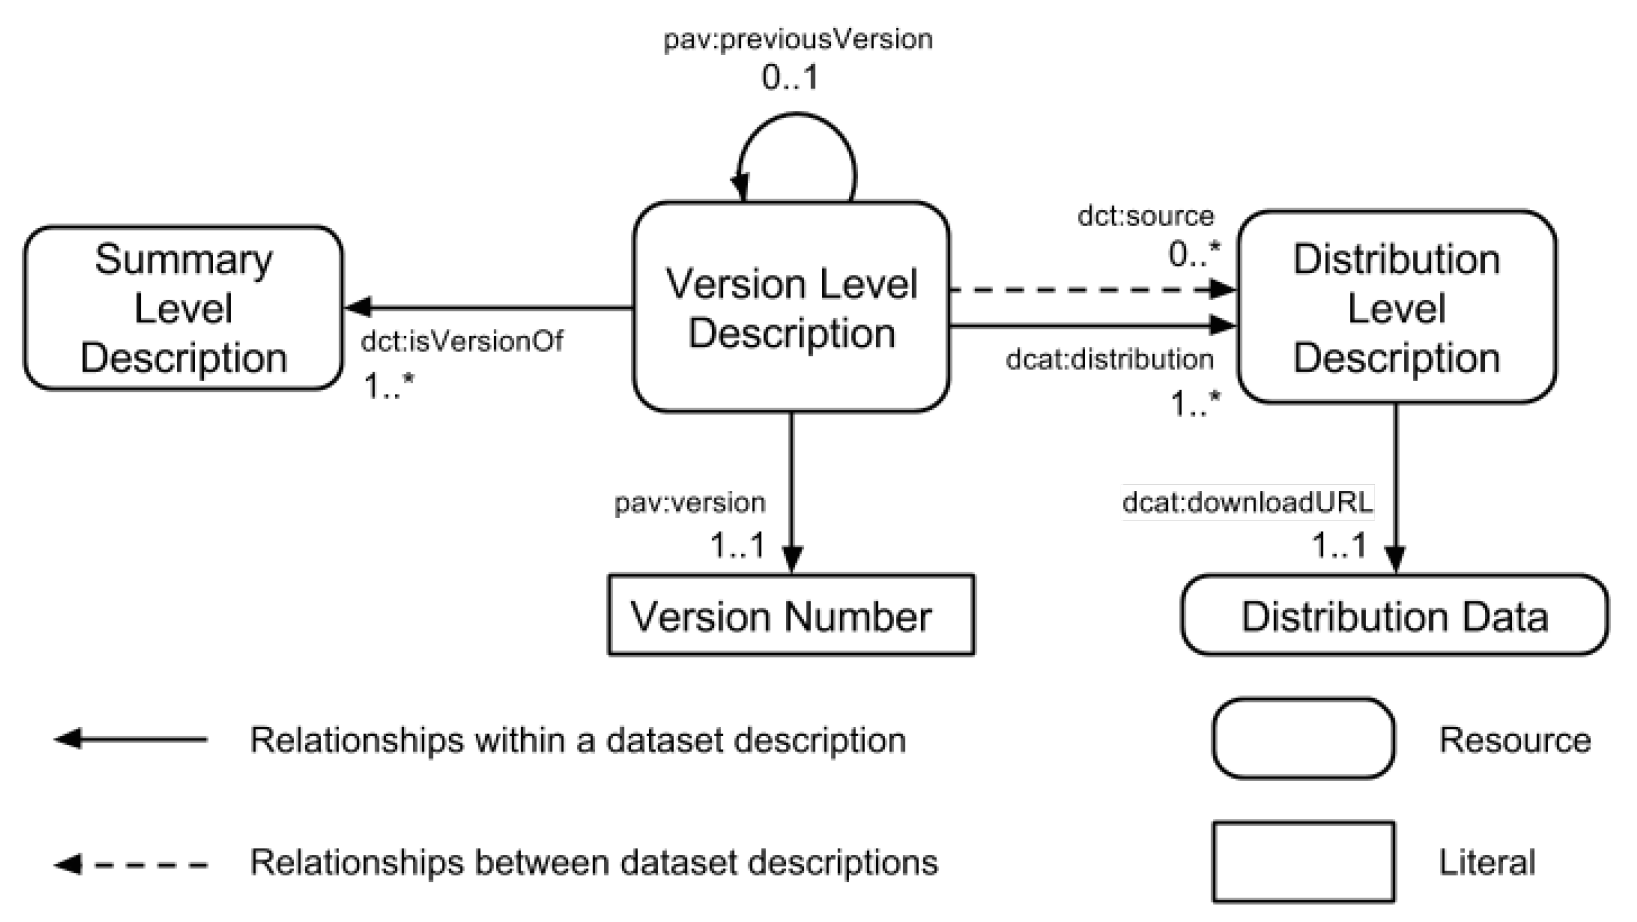
\includegraphics[scale=0.35]{figures/HCLSModel.png}
	\caption[Data model from the Health Care and Life Sciences Interest Group separating data into three levels: works, versions, and instances.]{Data model from the Health Care and Life Sciences Interest Group separating data into three levels: works, versions, and instances.  From Dummontier, et al. \cite{Dummontier2016}}
	\label{HCLSModel}
\end{figure}

\begin{figure}
	\centering
	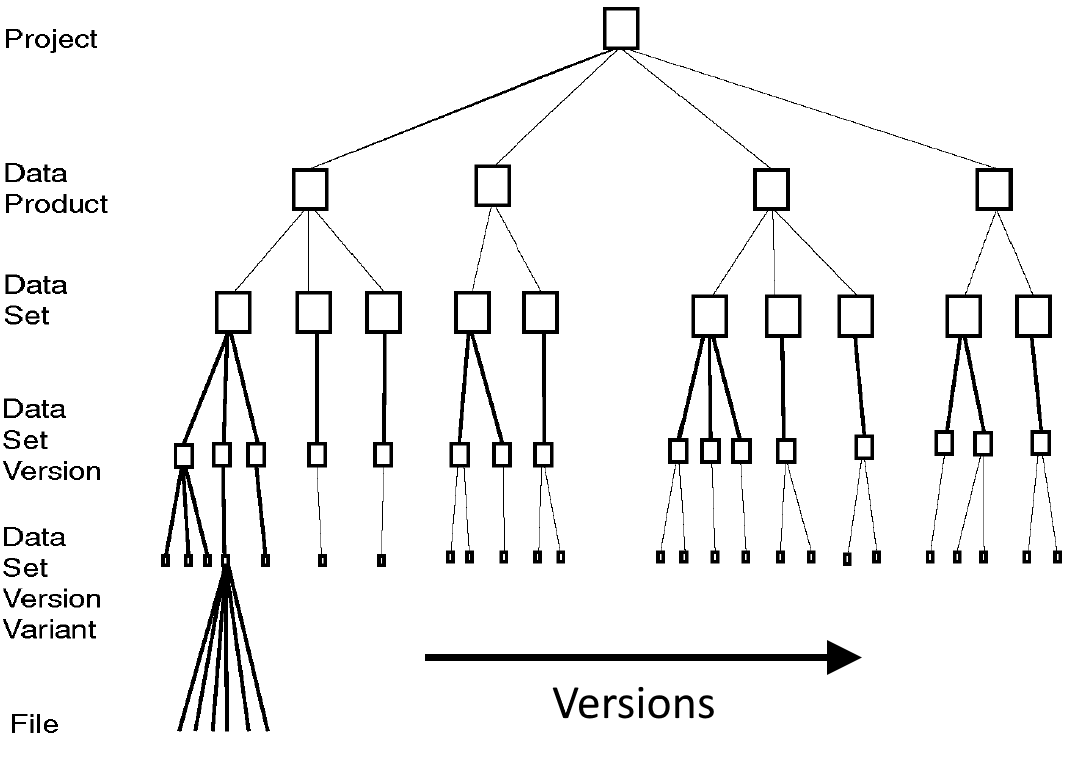
\includegraphics[scale=0.50]{figures/hierarchy.png}
	\caption[Visual representation of grouping hierarchy.]{Visual representation of grouping hierarchy.  From \cite{Barkstrom2003}}
	\label{hierarchy}
\end{figure}

The HCLS data model captures version information using the Provenance, Authoring, and Versioning (PAV) ontology \cite{Ciccarese2013}.
As explained in their document, PAV addresses versioning as a result of disagreements with other ontologies' definitions such as PROV.
They enumerate specific situations relating to health care data requiring broader conceptual coverage.
As a result, their model provides basic properties to identify a previous version and its corresponding identifier.
They do not provide methods to identify motivations or discuss the role attribute differences effect changing versions.
The existence and widespread adoption of change logs demonstrates the importance of this information in understanding modifications between versions.
However, PAV does adopt a state-based perspective regarding versioning since it only seeks to identify a previous version without attributing a responsible activity.

The PROV data model is a W3C recommendation which defines linked data properties to capture data provenance \cite{Gil2013}.
PROV has played a significant contribution in maintaining the quality and reproducibility of data sets and reporting in the National Climate Assessment (NCA) \cite{Ma2014191}.
This implication signifies that there is an increased likelihood of adoption through other scientific fields as a result of this reporting.
The Global Change Information System, which houses the data used to generate the NCA, uses PROV to meticulously track the generation of its artifacts and results as they are used in the report \cite{Tilmes2012}.
This means that not only does the data have a traceable lineage to verify quality, but the content of documents can have the same verifiability \cite{Ma2014}.
While a subtree of terms deal with versions, the ontology takes an activity based view of data.
This makes sense since it seeks to explain what activities led to the creation of an object.
This focus on activities results in a very shallow definition of methods to capture entity-to-entity relationships within the model.

\begin{figure}
	\centering
	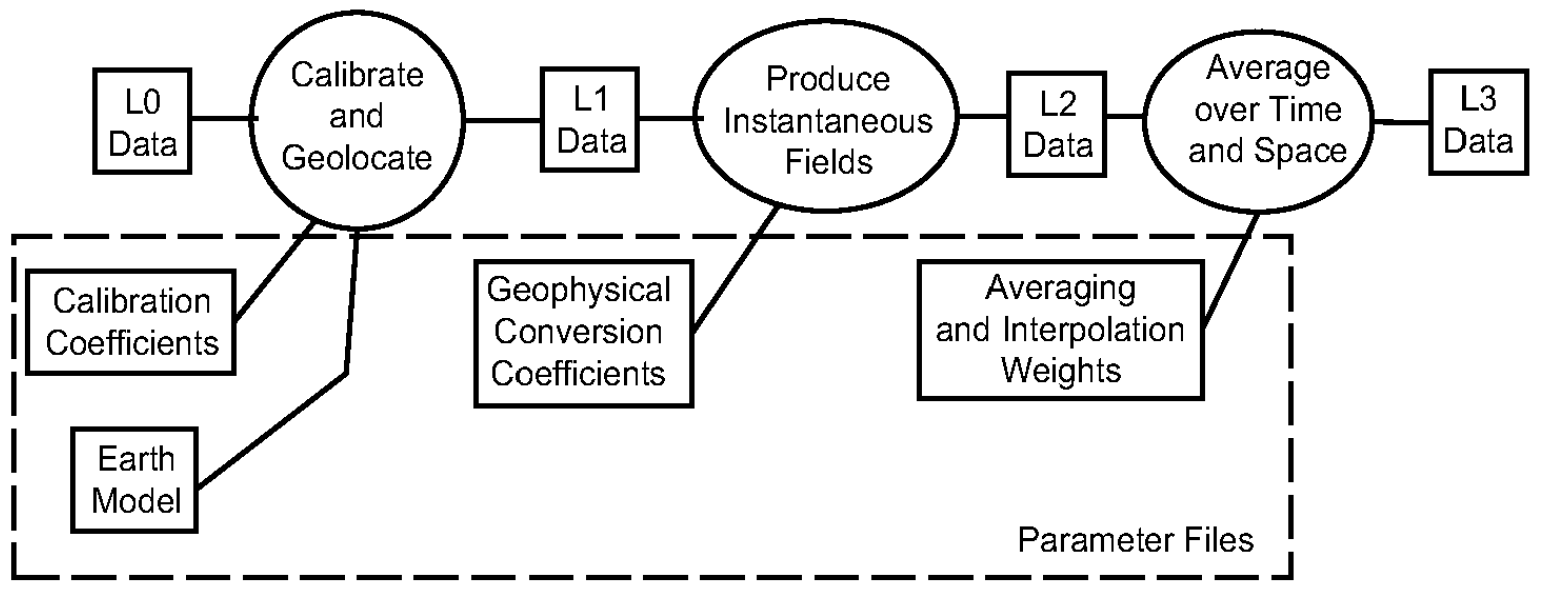
\includegraphics[scale=0.35]{figures/NASALevels.png}
	\caption[NASA organizes its data into three levels depending on the amount of aggregation and the distance the data is removed from the original sensor measurements.]{NASA organizes its data into three levels depending on the amount of aggregation and the distance the data is removed from the original sensor measurements. Figure 1 from \cite{Barkstrom2003}}
	\label{NASALevels}
\end{figure}

In his discourse on version management, Barkstrom introduces NASA's workflow model as seen in Figure \ref{NASALevels}.
It describes the formal stages of processing to turn a raw remote sensing signal from satellite instruments into global aggregate summaries \cite{Barkstrom2003}.
Understanding this model reveals that changes to either the algorithms or parameter files will force a change in the resulting data.
This explains the new result's provenance, but it would not capture the differences between these objects.
The key to understanding version modeling lies in recognizing provenance and versioning are intimately entwined, but seek to explain different properties about data objects.

There are two types of compatibility, `forwards', which explains how to modify old data to work with new content, and `backwards', which allows new data to interact with old data.
Knowing one type of compatibility does not always entail the means of deriving the other.
Having full forwards and backwards compatibility allows interoperability between a variety of applications which may use different versions of the same ontology.
However, it often depends on the application as to whether full compatibility is necessary.
Once concern which is very rarely discussed is the compatibility of files and objects which do not change at all.
They mention very little on how to migrate terms which do not change, but these can contribute to a majority of copied content and pose significant scaling issues.

\section{Provenance Ontologies}

The Proof Markup Language, one of the first semantic models to capture provenance information, expressed these relationships using inference reasoning through traceable graphs \cite{daSilva2006381}.

\subsection{Open Provenance Model}

A number of linked data models include versioning concepts such as the Open Provenance Model (OPM) \cite{moreau2008open}.
Driven by the uncertain needs and sometimes conflicting conventions of different scientific domains, the model sought to find a method to standardize the way in which provenance data is captured while also keeping the specification open to accommodate current data sets through the change.
In an experimental case, the model has been applied to sensor networks, automating and unifying their provenance capture even as they grow \cite{5478496}.
To aid OPM's adoption, the framework Karma2 integrates provenance capture into scientific workflows and provides a more abstract view of their data collection activities \cite{simmhan2010karma2}.
The property WasDerivedFrom constitutes a core concept in the model and marks the reliance of one object's existence on another object.
For a large part, this encompasses the engagement which provenance models view versions, without further need to explore the derivation's content.

\subsection{PROV-O}

PROV, a World Wide Web Consortium (W3C) Recommendation, delineates a method to express data provenance in a more compact form as seen in Figure \ref{PROVO} \cite{Gil2013a} \cite{Groth2013}.
The recommendation uses a conceptual model relating activities, agents, and entities to describe data production lineage \cite{Moreau2013c} \cite{Nies2013} \cite{Nies2013a}.
Intended as a high level abstraction, it takes an activity-oriented approach to provenance modeling.
Every data entity results from the actions of some activity.
The conceptual model's expression occurs through the PROV Ontology (PROV-O), which can be conveyed through various resource description languages \cite{Hua2013} \cite{Klyne2013}.
The ontology is further formalized into a functional notation for easier human consumption \cite{Moreau2013b} \cite{Cheney2013a}.
One particular strength that has contributed to the adoption of PROV is its ability to link into other ontologies, making it easier for existing semantically enriched data sets to adopt PROV \cite{Miles2013} \cite{Moreau2013}.
\begin{figure}
	\centering
	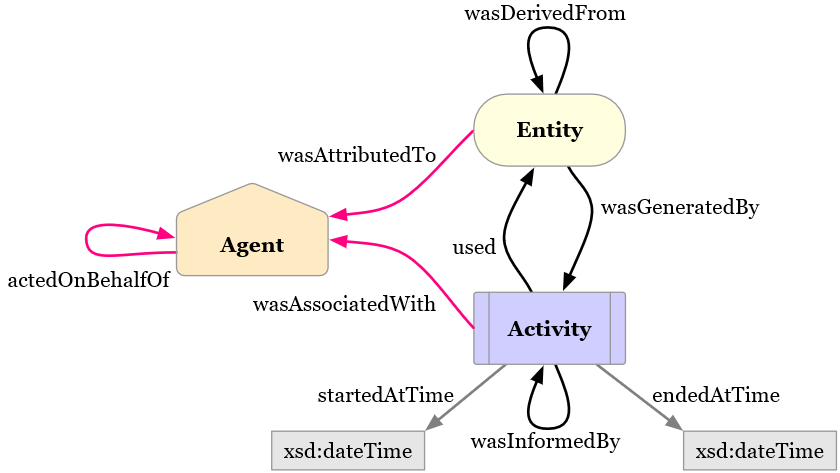
\includegraphics[scale=0.5]{figures/ProvO.png}
	\caption[Diagram of the PROV Ontology.]{Diagram of the PROV Ontology.  Figure 1 from \cite{Lebo2013}}
	\label{PROVO}
\end{figure}
Komadu, a framework developed to alleviate workflow integration, improves upon its predecessor, Karma, by no longer utilizing global context identifiers that were not necessarily shared throughout the workflow. \cite{Suriarachchi_2015}.

The PROV Ontology provides three different concepts that begin to encapsulate the provenance relationship between data versions.
It defines a \textit{prov:Generation} as "the completion of production of a new entity by an activity," \cite{Lebo2013}.
This means that the generation, which corresponds adding an object to a version, must result from a \textit{prov:Activity}.
\textit{Prov:Invalidation}, defined as the, ``start of the destruction, cessation, or expiry of an existing entity by an activity," makes a similar connection between activities and entities \cite{Lebo2013}.
A third concept, \textit{prov:Derivation}, relates two entities, and the ontology defines it as, "a transformation of an entity into another, an update of an entity resulting in a new one, or the construction of a new entity based on a preexisting entity. " \cite{Lebo2013}.
PROV also has a property called \textit{prov:isDerivedFrom} which conveys the same definition as a \textit{prov:Derivation}.
Using the property and concept together forms a qualified property which can be instantiated and further annotated.

\subsection{Provenance, Authorship, and Versioning Ontology}

The Provenance, Authorship, and Versioning (PAV) Ontology is, ``a lightweight vocabulary, for capturing ``just enough" descriptions essential for web resources representing digitized knowledge" \cite{Ciccarese2013}.
It provides a means to track versioning information through linked data by introducing \textit{pav:version} to cite versions and \textit{pav:previousVersion} to link them together in order \cite{Ciccarese2013}.
It does so in comparison to the Dublin Core concept \textit{dc:isVersionOf} which records, "Changes in version imply substantive changes in content rather than differences in format" \cite{DCMI2012}.
PAV supports the idea that a new concept becomes necessary to cover cases where new versions do not have to be substantive but can still be alternate editions of the original object.
While it documents related versions well, PAV does not dive deeper in explaining the circumstances behind version differences.

\subsection{Schema.org}

The Schema.org ontology is not a provenance ontology but provides a means to supply searchable web pages with standardized micro-data.
The ontology has a collection of concepts which could be applied to versioning.
The \textit{schema:UpdateAction} is defined as, ``the act of managing by changing/editing the state of the object," which encompasses the same responsibilities expected of versioning systems \cite{Schema}.
The terms \textit{schema:AddAction}, \textit{schema:DeleteAction}, and \textit{schema:ReplaceAction} subclass the \textit{shcema:UpdateAction}.
These classes model actions which further cement parallels between versioning and \textit{schema:UpdateAction}.

Schema.org defines a \textit{schema:ReplaceAction} as, ``the act of editing a recipient by replacing an old object with a new object" \cite{SchemaRep}.
The concept has two properties, \textit{schema:replacee} and \textit{schema:replacer} which indicates that a new object replaces an old one.
Schema.org models the interaction by placing the replacement action at the relation's center.
In comparison, the \textit{schema:AddAction} is defined as, ``the act of editing by adding an object to a collection" \cite{SchemaAdd}.
The action only involves the object and the new state of the collection, not involving any of the collection's prior lineage.
Schema.org defines the \textit{schema:DeleteAction} as, "the act of editing a recipient by removing one of its objects," \cite{SchemaRem}.
The concept aligns well with other versioning systems, although deletion may be a strong assertion.

\section{Thesis Statement}

Large data collection endeavors necessitate the development and deployment of versioning systems to manage change propagating through their data.
Advancing beyond identifier comparisons and delving into capturing substantive change can significantly improve the ability to standardize version communications and transition.
In chapter \ref{ch:prevwork}, we explore existing methods of codifying versions and change.
In chapter \ref{ch:model}, we define a model to provide a foundation in regularizing the versioning process and communicating that in a machine-computable manner using linked data.
In chapter \ref{ch:implement}, we implement the model and compare two methods in micro-data with JSON-LD expected to provide better performance.
These relations cannot be communicated by current provenance models' semantics.
Furthermore, in chapter \ref{ch:mbvl}, we show the model provides a quantitative basis for determining meaningful version identifiers following a numerical system which has previously only been performed using qualitative methods.
Through sub-classing concepts within this versioning model, versions can provide detailed comparisons to support experimental designs and decisions.


%%% Local Variables:
%%% mode: latex
%%% TeX-master: t
%%% End:
